\subsection{\sysname{}'s  Mechanism of \Kgroups  }
\label{comesh:section:design}

\sysname{} balances the STA load across space and time by using {\it \kgroups}---subgroups of smart devices,
monitoring devices and managing routines. 
A \kgroup{} is configured with a (system-wide)  parameter named $k$. To tolerate $f$ system-wide failures, we set $k = (2f+1)$.
We present  \kgroup{} internals (selection, election, quorum: \Cref{comesh:subsection:member_selection}),
temporal migration (\Cref{comesh:subsection:periodicity}), failure response  (\Cref{comesh:subsection:fault-tolerance}), and locality  (\Cref{comesh:subsection:lsh}).

\subsubsection{\Kgroup{} Operations: Selection, Leader, Quorum}
\label{comesh:subsection:member_selection}

\sysname's \kgroup{} selection needs to: (i) be load-balanced, and (ii) use a minimum number of messages. 
While some communication is unavoidable in any distributed system that aims to be fault-tolerant (e.g., pinging, membership, etc.), our key observation is that expensive distributed computing protocols
(e.g., leader election, member selection, etc.) can be replaced with inexpensive ``zero-message'' variants.

\noindent \textbf{Load-balanced Member Selection via Zero-message Exchange}: A smart device with ID $S$ discovers if it is present in a \kgroup{} for a target device with ID $D$ by calculating a consistent hash: $Hash (S, D)$~\cite{chord,dynamo}. The alphabetically {\it lowest} $k$ hashed IDs across the entire system are then the approved \kgroup{} members. This design is inspired by the idea of cryptographic sortition~\cite{cryptosort}.
Notice that, given a fixed hash function (e.g., a cryptographic hash like SHA-1), {\it any} arbitrary smart device can calculate the {\it entire} membership of {\it any} \kgroup{} by calculating this hash function on all known node IDs.
With correct membership lists, this takes zero messages.

\label{comesh:subsection:leadr_elctn}

\noindent{\bf Leader Election.}
The \kgroup{}'s goal is to fault-tolerantly replicate the state of its assigned entity (device or routine). To make its operations efficient, each \kgroup{} elects a leader, selected as that non-faulty \kgroup{} member with the lowest hashed value $Hash (S, D)$. 
Along with using the zero-exchange mechanism for election, \sysname{} ensures the leader is actually alive by running the (well-known)  
Bully election algorithm to quickly confirm the leader~\cite{Bully}. Bully election is attractive as it is fast in the common case: 1 RTT for lowest-hashed \kgroup{} device (leader) to inform others in the \kgroup{}.
Under failures Bully algorithm takes a worst case of 5 RTTs.

\label{comesh:subsection:quorum}

\noindent{\bf Quorum Agreement.} Fast agreement in a \kgroup{} is done via quorums. In a \kgroup{} of size $k=2\f+1$, anyone in a group (typically the leader) sends a message to all $M$ members, and waits for acknowledgments from at least $(\f+1)$ members. Thus with $\f$ failures, at least one surviving \kgroup{} member knows about the latest decisions in the \kgroup{}, and can communicate it to future leaders.

\subsubsection{Epoch-based \Kgroup{} Migration}
\label{comesh:subsection:periodicity}

While \Cref{comesh:subsection:member_selection}'s hashing provided  {\it spatial} load balance, for temporal load balancing, \sysname{}  migrates each \kgroup{} membership periodically.
Epoch lengths are fixed system-wide. (Different \kgroups{} can migrate at different times.)

\begin{algorithm}[t]
    \footnotesize
    \caption{\small \sysname{} \Kgroup{} Migration}
    \label{comesh:alg:migration}
    \algtext*{EndIf} % hide EndIf but keep block structure
    \algtext*{EndElse} % same for Else
    \begin{algorithmic}[1]
        \Require epoch $E$, current smart device $S$, smart device set $\mathcal{S}$, monitored device set $\mathcal{D}$, old \kgroup{} $\mathcal{M}_{old}$, old leader $L_{old}$
        \Ensure $\mathcal{D}$'s \kgroup{} migration
        \State $\mathcal{M}_{\mathcal{D}} \gets \text{calc\_members}(\text{++}E,\mathcal{D},\mathcal{S})$ \Comment{Using $Hash (E, S, D)$}
        \State $L_{\mathcal{D}} \gets \text{leader\_election}(\mathcal{M}_{\mathcal{D}})$
        \If{$S==L_{old}$}
            \State Replicate $state_{\mathcal{D}}$ to $L_{\mathcal{D}}$ \Comment{(a)}
            \State Receive and ack \texttt{CHANGEOVER} from $L_{\mathcal{D}}$ \Comment{(e)}
            \State Send \texttt{CHANGEOVER} to $\mathcal{M}_{old}$  \Comment{(f)}
        \ElsIf{$S==L_{\mathcal{D}}$}
            \State Receive $state_{\mathcal{D}}$ from $L_{old}$ \Comment{(b)}
            \State Replicate $state_{\mathcal{D}}$ to quorum of $\mathcal{M}_{\mathcal{D}}$ \Comment{(c)}
            \State Send \texttt{CHANGEOVER} to $L_{old}$ \Comment{(d)}
        \EndIf
    \end{algorithmic}
\end{algorithm}

First, we extend the hash function for the selection to include the epoch number $E$, making it $Hash (E, S, D)$. $E$ is incremented by 1 on each epoch change. When an epoch expires, \Cref{comesh:alg:migration} executes.
Epoch changes are initiated asynchronously by the leader of the old \kgroup{}.
When the new \kgroup{} leader acknowledges to the old \kgroup{} leader 
that it has received all the state (line 5), the old \kgroup{} leader can delete its old \kgroup{} state. After line 6, an old \kgroup{} node can delete its old state for that \kgroup{}. During \Cref{comesh:alg:migration}'s execution,
no monitoring operations occur in the \kgroup{}. This means that old \kgroup{} members and the old leader cease all \kgroup{} operations at exactly the epoch changeover boundary. In practice, the epoch change is fast enough that this gap in monitoring
is small, as shown by our experimental results.
After the migration, all normal \kgroup{} operations resume. 

\subsubsection{Failure Response: \Kgroup{} Updates}
\label{comesh:subsection:fault-tolerance}

If a device $N_i$ fails, the decentralized failure detector layer informs all other smart devices of its failure. Because \sysname{}'s operations remain correct for group size $k \in [f+1, 2f+1]$ (a majority is still present), we trigger a \kgroup{} update only when $f$ smart devices have failed (rather than on each failure)---this keeps the overhead of failure response low.

If the failed device $N_i$ was a leader of a \kgroup{},  this triggers  \Cref{comesh:subsection:leadr_elctn}'s election.  
This new leader needs to reconstruct the state from all the members in the \kgroup{}. This state is correct because of past quorums across
at least $f+1$ \kgroup{} members, so the new leader receives each past update from at least one non-faulty member.
Once reconstructed, the leader sends this state to the \kgroup{} and waits for confirmation by a quorum ($f+1$). 
If the new leader fails during reconstruction, the election is re-run, and this process repeats.

\subsubsection{Grouping and Locality-Sensitive Hashing}
\label{comesh:subsection:lsh}

Since \sysname{} is running over an ad-hoc network, two  issues arise: 
(i) the sheer number of devices and routines creates too many \kgroup{}s,  
(ii) if \kgroup{} members are randomly selected (hashed), they will be spread out, making intra-\kgroup{} coordination slow and bandwidth-hungry.

\noindent {\bf 1. Limiting the Number of \Kgroup{}s:} We use a
genetic k-means clustering algorithm~\cite{KMeans} to group the devices. Each resultant device group is assigned to one \kgroup. For routines, we pick a random device from its trigger set as its representative, and that device's \kgroup{} becomes the routine's \kgroup. 

\noindent {\bf 2. Locality-Sensitive Hashing: } Selecting \kgroup{}s randomly (\Cref{comesh:subsection:member_selection}) spreads the \kgroup{} members all over the network, slowing down
{both intra-group (election, quorum) and inter-leader operations}.
A challenge is to make \kgroup{} selection {\it local} while retaining spatial load-balancing benefits of hashing. %To do so, w
We use physical device locations and adapt ideas from {\it locality-sensitive hashing (LSH)}~\cite{datar_locality-sensitive_2004}. 
In IoT, LSH has been used for flows~\cite{iottraffic} and outlier detection~\cite{omnibus}, but \sysname{} is the first to adapt LSH for coordination protocols. Our LSH-based selection is compatible with zero message exchange protocols described earlier (\Cref{comesh:subsection:member_selection}).
Classical LSH~\cite{datar_locality-sensitive_2004} hashes similar multi-dimensional vectors into the same ``buckets'' with high probability. 
\Cref{comesh:alg:lsh_majority_selection} details how \sysname{} selects a device \kgroup's $f{+}1$ majority using LSH.

\begin{algorithm}[t]
    \footnotesize
    \caption{\small \sysname{} LSH Majority Selection Rule}
    \label{comesh:alg:lsh_majority_selection}
    \algtext*{EndIf} % hide EndIf but keep block structure
    \algtext*{EndElse} % same for Else
    \begin{algorithmic}[1]
        \Require Monitored device set $\mathcal{D}$, smart device set $\mathcal{S}$
        \Ensure Selected smart device list $R$ of size $f + 1$
        \State Initialize $N \gets$ a random device in $\mathcal{D}$
        \State $\{B_{\mathcal{S}_i}\} \gets \{\text{LSH}(\mathcal{S}_i)\}$ for all $\mathcal{S}_i \in \mathcal{S}$ \Comment{buckets}
        \State $B_{N} \gets \text{LSH}(N)$
        \State $R \gets$ $\{\mathcal{S}_i\}$ where $B_{\mathcal{S}_i} = B_{N}$ \Comment{same bucket}
        \If{$\text{size}(R) \leq f + 1$}
            \State $B_{\text{neigh}} \gets \text{LSH}(\text{neighbors of } N)$
            \State $R \gets R  \cup \text{smart devices in }B_{\text{neigh}}$
        \EndIf
        \If{$\text{size}(R) > f + 1$} Truncate $R$ to size $f + 1$
        \Else{} Add random smart devices to $R$ until size($R$) = $f + 1$
        \EndIf
        \State \Return $R$
    \end{algorithmic}
\end{algorithm}

At each epoch, we also desire a \kgroup{} to migrate only ``nearby'' so that STA traffic stays local, and state transfer to new \kgroup{} is fast.

The device's location vector is $d$-dimensional and the \textit{state vector} of a smart device is a $2d$-dimensional vector that combines the device's location with the average location of all devices it monitors, to preserve locality. 
For example, let $d = 2$ and $(x_{S_i}, y_{S_i})$ denote smart device $S_i$'s coordinates. Let $\{(x_j, y_j)\}_{j=1}^m$ represent the coordinates of the $m$ devices monitored by $S_i$ during a given epoch. The averaged location of the monitored devices is:
$ 
% \[
x_{\text{ave}} = \frac{1}{m} \sum_{j=1}^{m} x_j, \quad y_{\text{ave}} = \frac{1}{m} \sum_{j=1}^{m} y_j
% \]
$.
Thus, the \textit{state vector} of smart device $S_i$ at this epoch is:
% \[
$
(x_{S_i},\ y_{S_i},\ x_{\text{ave}},\ y_{\text{ave}})
$.
% \]
For simple devices, we append the location vector $(x_1, \dots, x_d)$ so that all devices have the same dimensions for LSH. 

\sysname{} uses the LSH function $h_{\bm{a},b} = \lfloor{ \frac{\bm{a}\cdot\bm{v}+b}{r}} \rfloor$, adapted from~\cite{datar_locality-sensitive_2004}.
To reduce the probability of differing vectors being bucketed together, \sysname{} includes two further optimizations: (i) concatenate hash functions, i.e., $H = (h_1, ..., h_m)$); and (ii) use multiple ($l$) hashes. Thus \sysname{} uses $\mathcal{H} = \{H_1,..., H_l\} =\{(h_{11}, ..., h_{1m}),..., (h_{l1}, ..., h_{lm})\}$.
\Cref{comesh:tab:lsh_params} summarizes the aforementioned LSH parameters.

\begin{table}[t]
    \centering
    \caption{\small \it Summary of LSH parameters used in \sysname.}
    \bigskip
    \label{comesh:tab:lsh_params}
    % \tagpdfsetup{table/header-rows={1},table/header-columns={1}}
    \tagpdfsetup{table-tagging=false}
    \setlength{\tabcolsep}{4pt}
    \begin{tabular}{c l c}
        \hline
        \textbf{Symbol}   & \textbf{Definition}   & \textbf{Default} \\ \hline
        \( a \)           & Random Gaussian vector, same dimension as \(v\)~\cite{zolotarev1986onedimensional} & --- \\
        \( b \)           & Uniform scalar in \([0, r)\)           & --- \\
        \( r \)           & Size of quantization interval          & 4   \\
        \( m \)           & Number of concatenated hash functions  & 2   \\
        \( l \)           & Number of independent hash groups      & 2   \\ \hline
    \end{tabular}
\end{table}

\begin{figure}[tb!]
    \centering
    \begin{subfigure}[b]{0.4\linewidth}
        \centering
        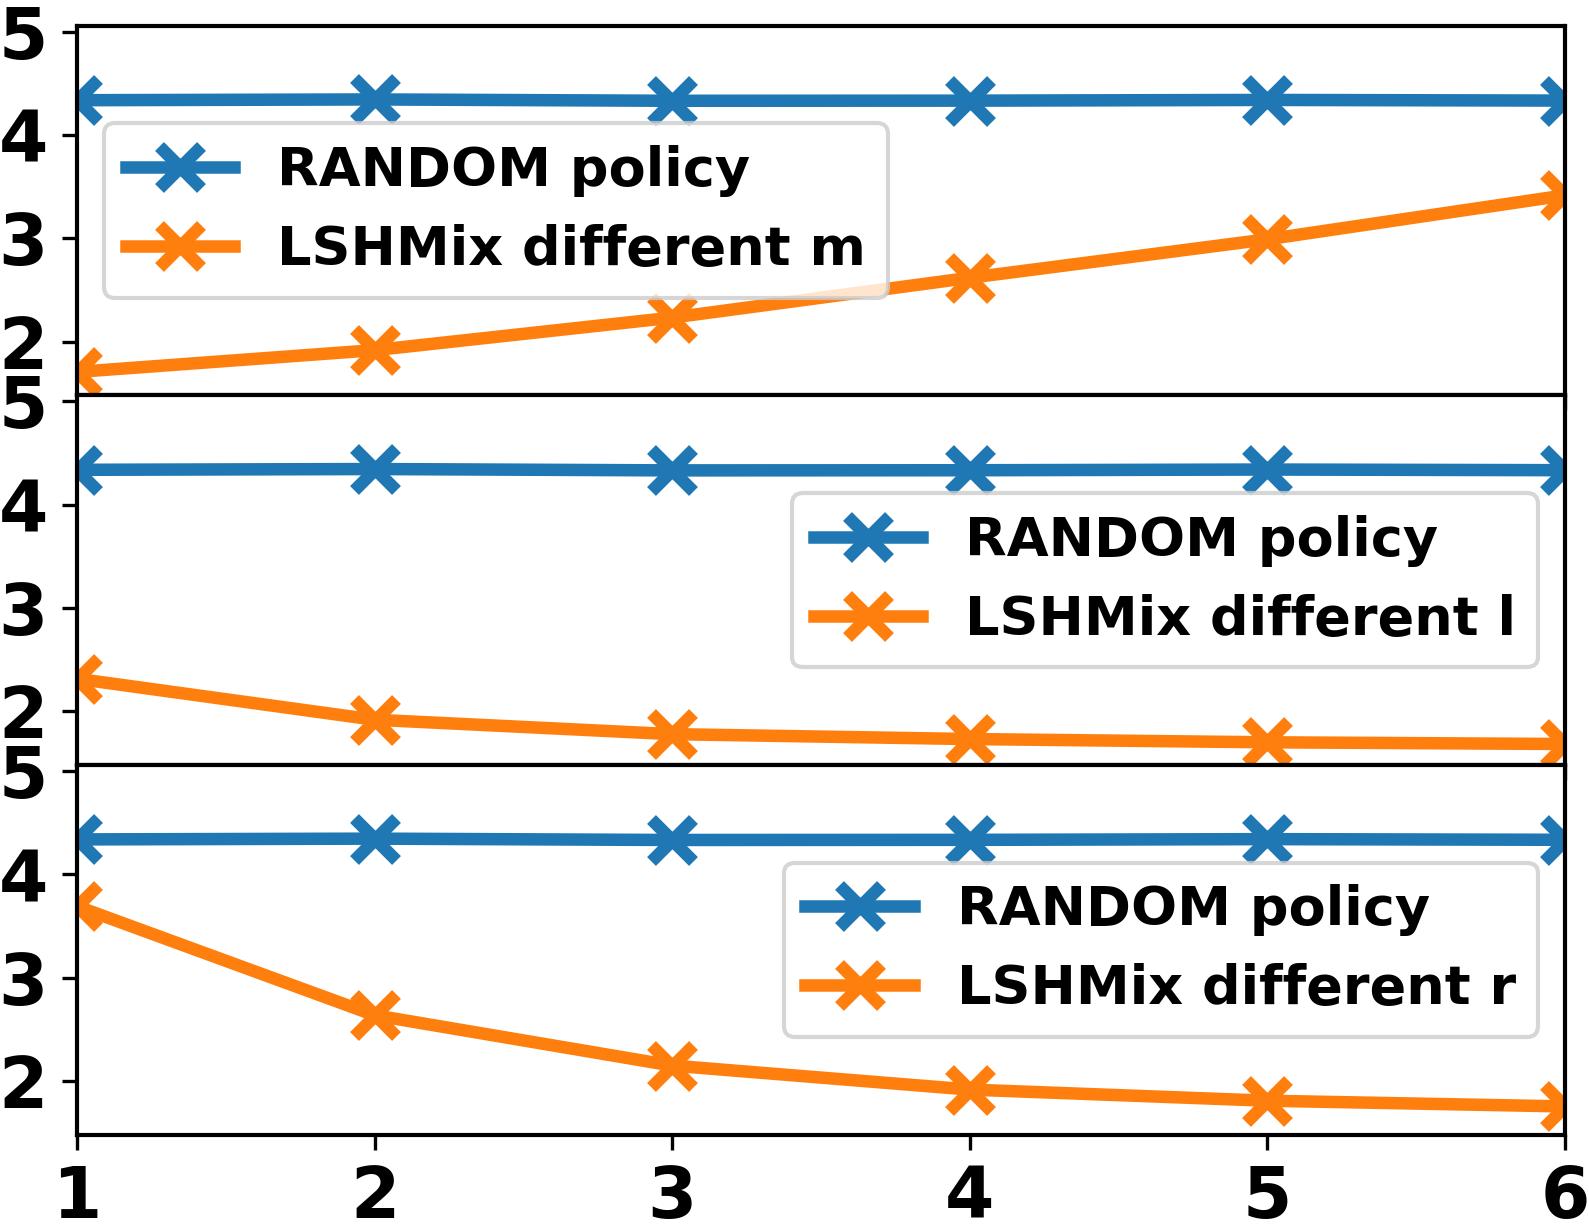
\includegraphics[width=\textwidth]{CoMesh/figures/k-groups/500_grid5,10,10lsh_kdis_k_l_r.png}
        \caption{\small \it Average quorum distance.}
        \label{comesh:subfig:quorum_dis_500klr}
    \end{subfigure}
    \hspace{0.5cm}
    \begin{subfigure}[b]{0.4\linewidth}
        \centering
        \hspace{-8pt}
        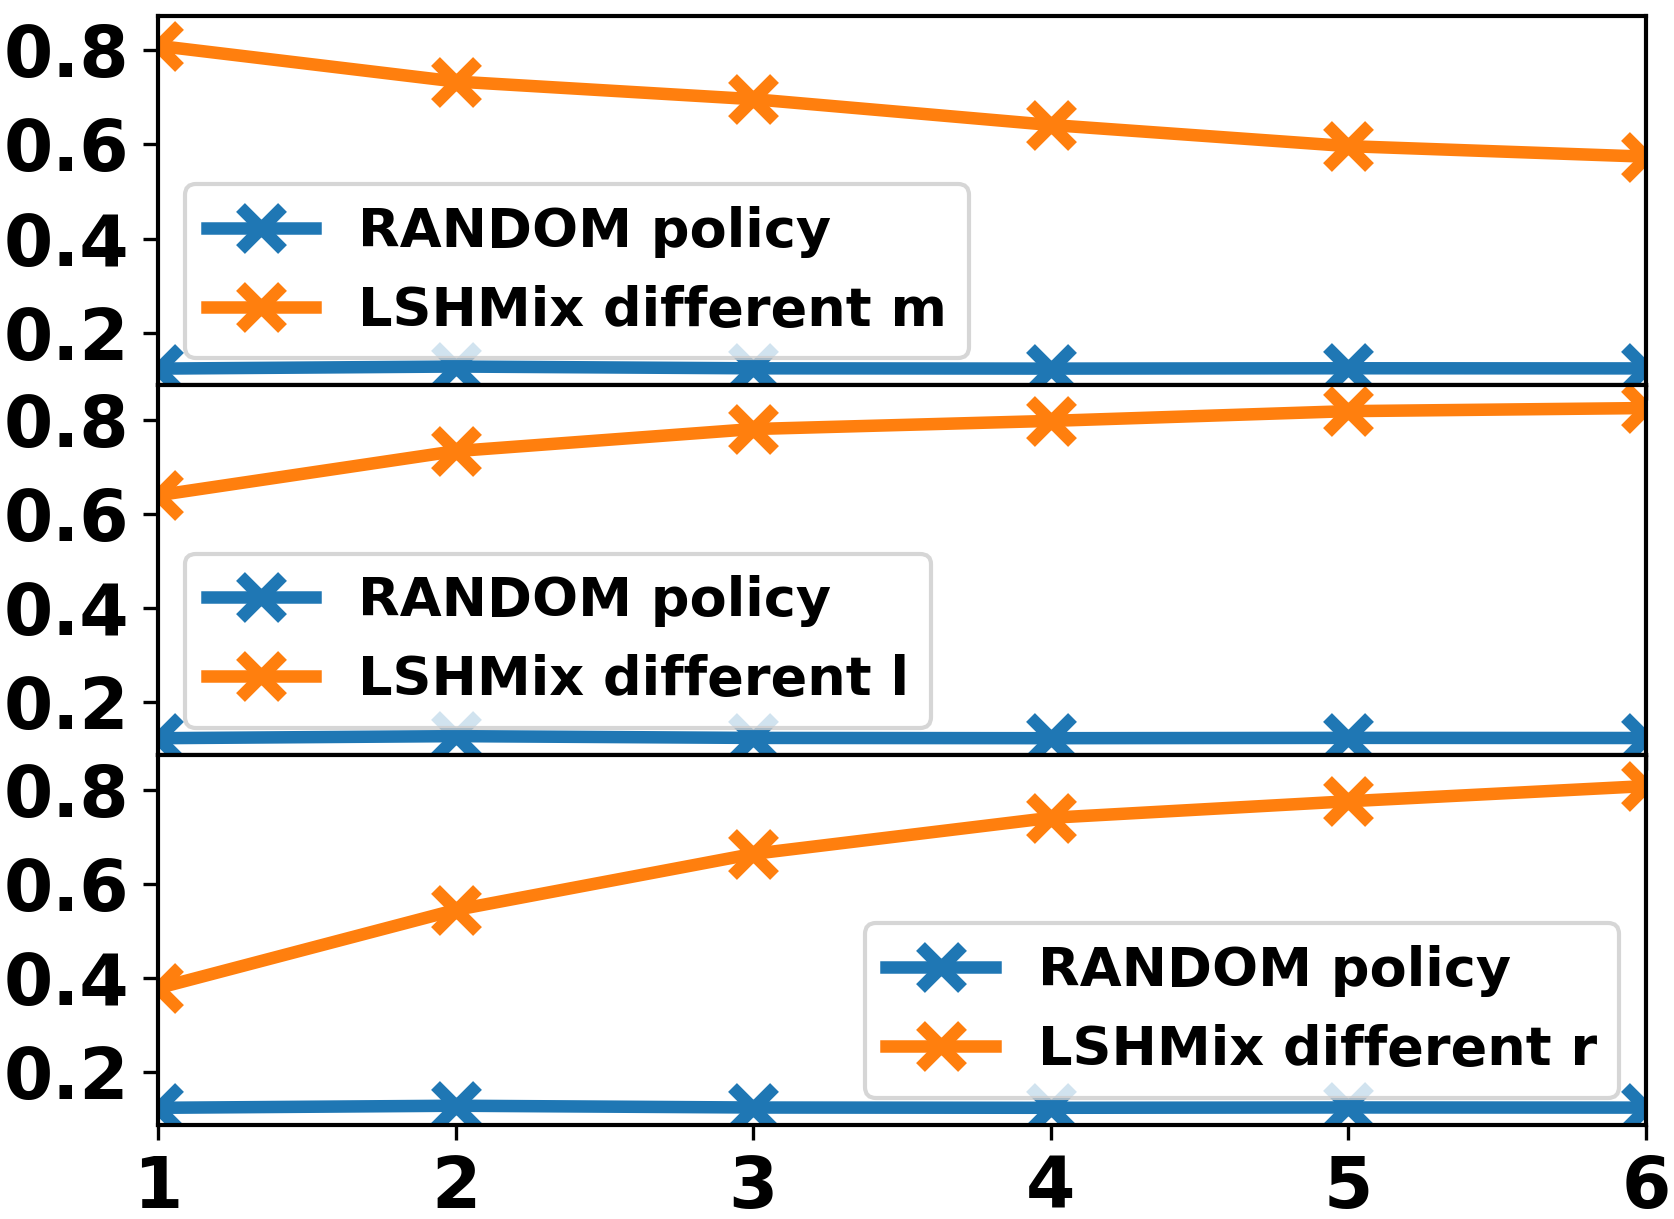
\includegraphics[width=1.04\textwidth]{CoMesh/figures/k-groups/500_grid5,10,10lsh_koverlap_k_l_r.png}
        \caption{\small \it Average \kgroup{} overlap.}
        \label{comesh:subfig:overlap_500klr}
    \end{subfigure}
    \caption{\small \it Average quorum distance and \kgroup{} overlap for different selection policies and parameters. $N$ = 500, \#smart devices = 200.}
    \medskip
    \label{comesh:fig: ave_quorum_dis_and_overlap_klr}
\end{figure}

\Cref{comesh:subfig:quorum_dis_500klr,comesh:subfig:overlap_500klr} show that increasing $m$
over-clusters devices while raising $l,r$ does the reverse. By default \sysname{} sets $m=2, l=2, r=4$.
This has clear benefits---our results 
show that in 2D grid topologies of different sizes,  LSH has a smaller intra-group quorum distance than random \kgroup{} selection. 

